\section{eo\-NDSorting\_\-I$<$ EOT $>$ Class Template Reference}
\label{classeo_n_d_sorting___i}\index{eoNDSorting_I@{eoNDSorting\_\-I}}
The original Non Dominated Sorting algorithm from Srinivas and Deb.  


{\tt \#include $<$eo\-NDSorting.h$>$}

Inheritance diagram for eo\-NDSorting\_\-I$<$ EOT $>$::\begin{figure}[H]
\begin{center}
\leavevmode
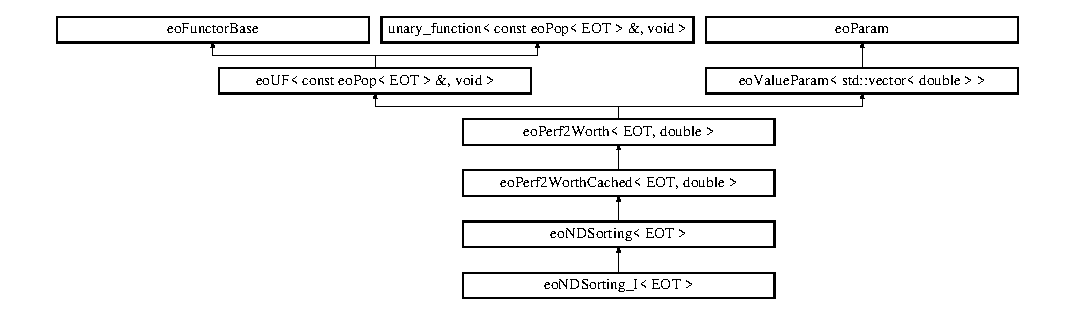
\includegraphics[height=3.78378cm]{classeo_n_d_sorting___i}
\end{center}
\end{figure}
\subsection*{Public Member Functions}
\begin{CompactItemize}
\item 
{\bf eo\-NDSorting\_\-I} (double \_\-niche\-Size, bool nasty\_\-flag\_\-=false)\label{classeo_n_d_sorting___i_a0}

\item 
std::vector$<$ double $>$ {\bf niche\_\-penalty} (const std::vector$<$ unsigned $>$ \&current\_\-front, const {\bf eo\-Pop}$<$ {\bf EOT} $>$ \&\_\-pop)
\begin{CompactList}\small\item\em Pure virtual function that calculates the 'distance' for each element in the current front Implement to create your own nondominated sorting algorithm. \item\end{CompactList}\end{CompactItemize}
\subsection*{Private Attributes}
\begin{CompactItemize}
\item 
double {\bf niche\-Size}\label{classeo_n_d_sorting___i_r0}

\end{CompactItemize}


\subsection{Detailed Description}
\subsubsection*{template$<$class EOT$>$ class eo\-NDSorting\_\-I$<$ EOT $>$}

The original Non Dominated Sorting algorithm from Srinivas and Deb. 



Definition at line 380 of file eo\-NDSorting.h.

\subsection{Member Function Documentation}
\index{eoNDSorting_I@{eo\-NDSorting\_\-I}!niche_penalty@{niche\_\-penalty}}
\index{niche_penalty@{niche\_\-penalty}!eoNDSorting_I@{eo\-NDSorting\_\-I}}
\subsubsection{\setlength{\rightskip}{0pt plus 5cm}template$<$class EOT$>$ std::vector$<$double$>$ {\bf eo\-NDSorting\_\-I}$<$ {\bf EOT} $>$::niche\_\-penalty (const std::vector$<$ unsigned $>$ \& {\em current\_\-front}, const {\bf eo\-Pop}$<$ {\bf EOT} $>$ \& {\em \_\-pop})\hspace{0.3cm}{\tt  [inline, virtual]}}\label{classeo_n_d_sorting___i_a1}


Pure virtual function that calculates the 'distance' for each element in the current front Implement to create your own nondominated sorting algorithm. 

The size of the returned std::vector should be equal to the size of the current\_\-front. 

Implements {\bf eo\-NDSorting$<$ EOT $>$} {\rm (p.\,\pageref{classeo_n_d_sorting_a2})}.

Definition at line 385 of file eo\-NDSorting.h.

The documentation for this class was generated from the following file:\begin{CompactItemize}
\item 
eo\-NDSorting.h\end{CompactItemize}
